% !TeX program = lualatex
% !TeX encoding = utf8
% !TeX spellcheck = english
% !TeX root =../MexPractEng.tex

%=========================================================
\chapter{Mechanical Oscillations}\label{\currfilebase}
\Opensolutionfile{answer}[\currfilebase/\currfilebase-Answers]
\Writetofile{answer}{\protect\section*{\nameref*{\currfilebase}}}%
%=========================================================

\section{Kinematics of Simple Harmonic Motion}


%=========================================================
\begin{problem}
	A simple harmonic oscillator takes $12.0$~s to undergo five
	complete vibrations. Find 
	\begin{enumerate*}[label=(\alph*)]
		\item the period of its motion,
		\item the frequency in hertz, and
		\item the angular frequency in radians per second.
	\end{enumerate*}
\end{problem}

%=========================================================
\begin{problem}
	A object with mass $0.500$~kg attached to a spring with a force constant of $8.00$~N/m vibrates in simple harmonic motion with an amplitude of $10.0$~cm. Calculate the maximum value of its 
	\begin{enumerate*}[label=(\alph*)]
		\item speed and
		\item acceleration, 
		\item the speed and
		\item the acceleration when the object is $6.00$~cm from the equilibrium position, and 
		\item the time interval required for the object to move from $x = 0$ to $x = 8.00$~cm.
	\end{enumerate*}
	\begin{solution}
		\begin{enumerate*}[label=(\alph*)]
		\item $40.0$~\si{\centi\meter\per\second}; 
		\item $160$~\si{\centi\meter\per\square\second};
		\item $32.0$~\si{\centi\meter\per\second};
		\item $296.0$~\si{\centi\meter\per\square\second};
		\item $0.232$~s. 
		\end{enumerate*}
	\end{solution}
\end{problem}


%=========================================================
\begin{problem}
	In an engine, a piston oscillates with simple harmonic
	motion so that its position varies according to the
	expression
	\[
		x= 5.00 \cos\left(2 t +\frac{\pi}{6}\right)
	\]
	where $x$ is in centimeters and $t$ is in seconds. At $t = 0$, find
	\begin{enumerate*}[label=(\alph*)]
		\item the position of the particle, 
		\item its velocity, and 
		\item its acceleration.
		Find
		\item the period and
		\item the amplitude of the motion.
	\end{enumerate*}
\end{problem}


%=========================================================
\begin{problem}
	A $1.00$~kg object is attached to a horizontal spring. The spring is initially stretched by $0.100$~m, and the object is released from rest there. It proceeds to move without friction. The next time the speed of the object is zero is $0.500$~s later. What is the maximum speed of the object?
	\begin{solution}
		$0.628$\si{\meter\per\second}.
	\end{solution}
\end{problem}

%=========================================================
\begin{problem}\label{prb:osc_x(t)}
	An object attached to a spring vibrates with simple harmonic motion as described by Figure~\ref{osc_x(t)}. For this motion, find
	\begin{enumerate*}[label=(\alph*)]
		\item the amplitude,
		\item the period,
		\item the angular frequency,
		\item the maximum speed,
		\item the maximum acceleration, and
		\item an equation for its position x as a function of time.
	\end{enumerate*}
\end{problem}


%=========================================================
\begin{problem}\label{prb:osc_v(t)}
	What is the phase constant for the harmonic oscillator with the velocity function $v(t)$ given in Fig.~\ref{osc_v(t)} if the position function $x(t)$ has the form 
	\[
	x = A\cos(\omega t +\phi)
	\]
\end{problem}

%=========================================================
\begin{figure}[h!]\centering
	%---------------------------------------------------------
	\begin{minipage}[t]{0.45\linewidth}\centering
	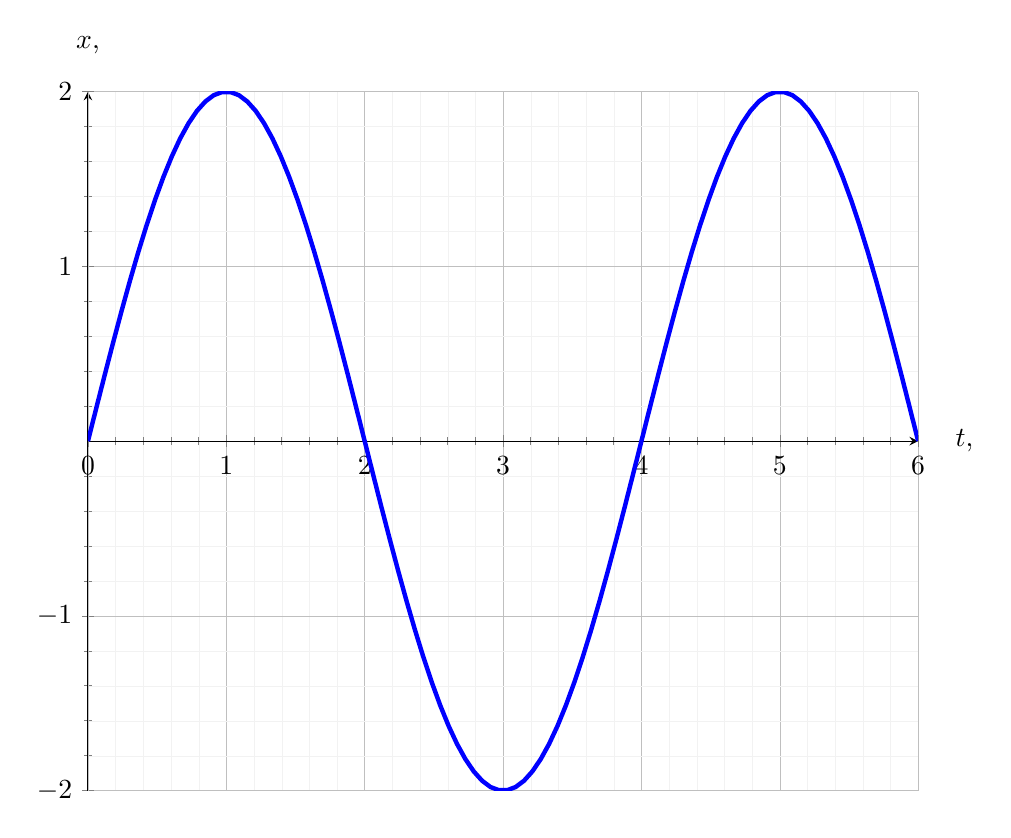
\begin{tikzpicture}
		\begin{axis}[%
		% === Налаштування сітки ===
		grid = both,
		grid style={line width=.1pt, draw=gray!10},
		major grid style={line width=.2pt,draw=gray!50},
		minor tick num = 4,
		minor grid style = {line width=.1pt,draw=gray!10},
		% === Налаштування положення координатних осей ===
		axis lines = middle,
		axis line style={-stealth},
		% === Вибір підписів шкали для відображення ===
		xtick = {0,1,...,6},
		extra x ticks=0,
		ytick = {-2,-1,...,2},
		% === Підпис координатних осей ===
		ylabel={$x$, \si{\meter}},
		xlabel={$t$, \si{\second}},
		% === Положення підпису координатних осей ===
		xlabel style={right = 10pt},
		ylabel style={above = 10pt},
		% === Налаштування мінімальних та максимальних значень координат ===
		xmin = 0,
		xmax =  6,
		ymin = -2,
		ymax =  2,
		% === Налаштування розміру графіка ===
		width=\linewidth,
		]
		\addplot+[blue, no marks, domain={0:6}, samples=100, ultra thick] {2*sin(deg(2*pi/4*x))};
		\end{axis}
		\end{tikzpicture}
		\caption{Problem~\ref{prb:osc_x(t)}}
		\label{osc_x(t)}
	\end{minipage}
	%---------------------------------------------------------
	\begin{minipage}[t]{0.45\linewidth}\centering
		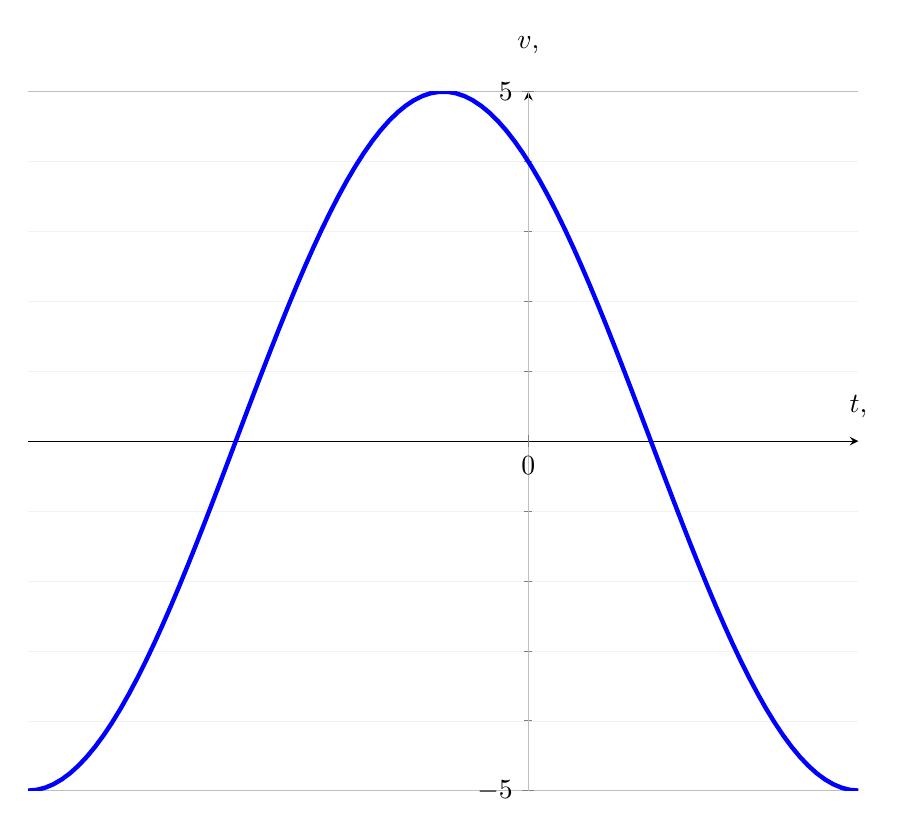
\begin{tikzpicture}
		\begin{axis}[%
		% === Налаштування сітки ===
		grid = both,
		grid style={line width=.1pt, draw=gray!10},
		major grid style={line width=.2pt,draw=gray!50},
		minor tick num = 4,
		minor grid style = {line width=.1pt,draw=gray!10},
		% === Налаштування положення координатних осей ===
		axis lines = middle,
		axis line style={-stealth},
		% === Вибір підписів шкали для відображення ===
		xtick = \empty,
		extra x ticks=0,
		ytick = {-5,0,5},
		% === Підпис координатних осей ===
		ylabel={$v$, \si{\centi\meter\per\second}},
		xlabel={$t$, \si{\second}},
		% === Положення підпису координатних осей ===
		xlabel style={above = 5pt},
		ylabel style={above = 10pt},
		% === Налаштування мінімальних та максимальних значень координат ===
		xmin = {-pi - pi/180*acos(4/5)},
		xmax =  {pi - pi/180*acos(4/5)},
		ymin = -5,
		ymax =  5,
		% === Налаштування розміру графіка ===
		width=\linewidth,
		]
		\addplot+[blue, no marks, domain={{-pi - pi/180*acos(4/5)}:{pi - pi/180*acos(4/5)}}, samples=100, ultra thick] {5*cos(deg(x) + acos(4/5))};
		\end{axis}
		\end{tikzpicture}
		\caption{Problem~\ref{prb:osc_v(t)}}
		\label{osc_v(t)}
	\end{minipage}
	%---------------------------------------------------------
\end{figure}
%=========================================================
%=========================================================
\begin{problem}
	A particle with a mass of $1.00 \cdot 10^{-20}$~kg is oscillating with simple harmonic motion with a period of $1.00 \cdot 10^{-5}$~s and a maximum speed of $1.00 \cdot 10^3$~m/s. Calculate 
	\begin{enumerate*}[label=(\alph*)]
		\item the angular frequency and
		\item the maximum displacement of the particle.
	\end{enumerate*}
\end{problem}


\section{Energy of the Simple Harmonic Oscillator}


%=========================================================
\begin{problem}
	A $50.0$~g object connected to a spring with a force constant of $35.0$~N/m oscillates with an amplitude of $4.00$~cm on a frictionless, horizontal surface. Find 
	\begin{enumerate*}[label=(\alph*)]
		\item the total energy of the system and
		\item the speed of the object when its position is $1.00$~cm.
		Find
		\item the kinetic energy and
		\item the potential energy when its position is $3.00$~cm.
	\end{enumerate*}
	\begin{solution}
		\begin{enumerate*}[label=(\alph*)]
			\item $28.0$~mJ; 
			\item $1.02$~m/s; 
			\item $12.2$~mJ;
			\item $15.8$~mJ.
		\end{enumerate*}
	\end{solution}
\end{problem}

%=========================================================
\begin{problem}
	A simple harmonic oscillator of amplitude $A$ has a total energy $E$. 
	Determine 
	\begin{enumerate*}[label=(\alph*)]
		\item the kinetic energy and
		\item the potential energy when the position is one-third the amplitude.
		\item For what values of the position does the kinetic energy equal one-half the potential energy?
		\item Are there any values of the position where the kinetic energy is greater than the maximum potential energy?
	\end{enumerate*}
	\begin{solution}
		\begin{enumerate*}[label=(\alph*)]
			\item $\frac{8}{9} E$;
			\item $\frac{1}{9} E$;
			\item $x = \pm \sqrt{\frac23} A$.
		\end{enumerate*}
	\end{solution}
\end{problem}


%=========================================================
\begin{problem}\label{prb:osc_U(x)}
	Figure~\ref{osc_U(x)} gives the one dimensional potential energy well for a $2.0$~kg particle. 
	\begin{enumerate*}[label=(\alph*)]
		\item If the particle passes through the equilibrium position with a velocity of $85$~cm/s, will it be turned back before it reaches $x = 15$~cm?
		\item If yes, at what position, and if no, what is the speed of the particle at $x = 15$~cm?
	\end{enumerate*}
\end{problem}


%=========================================================
\begin{problem}\label{prb:osc_K(x)}
	Figure~\ref{osc_K(x)} shows the kinetic energy $K$ of a simple harmonic oscillator versus its position $x$. What is the spring constant?
\end{problem}

%=========================================================
\begin{figure}[h!]\centering
	%---------------------------------------------------------
	\begin{minipage}[t]{0.45\linewidth}\centering
		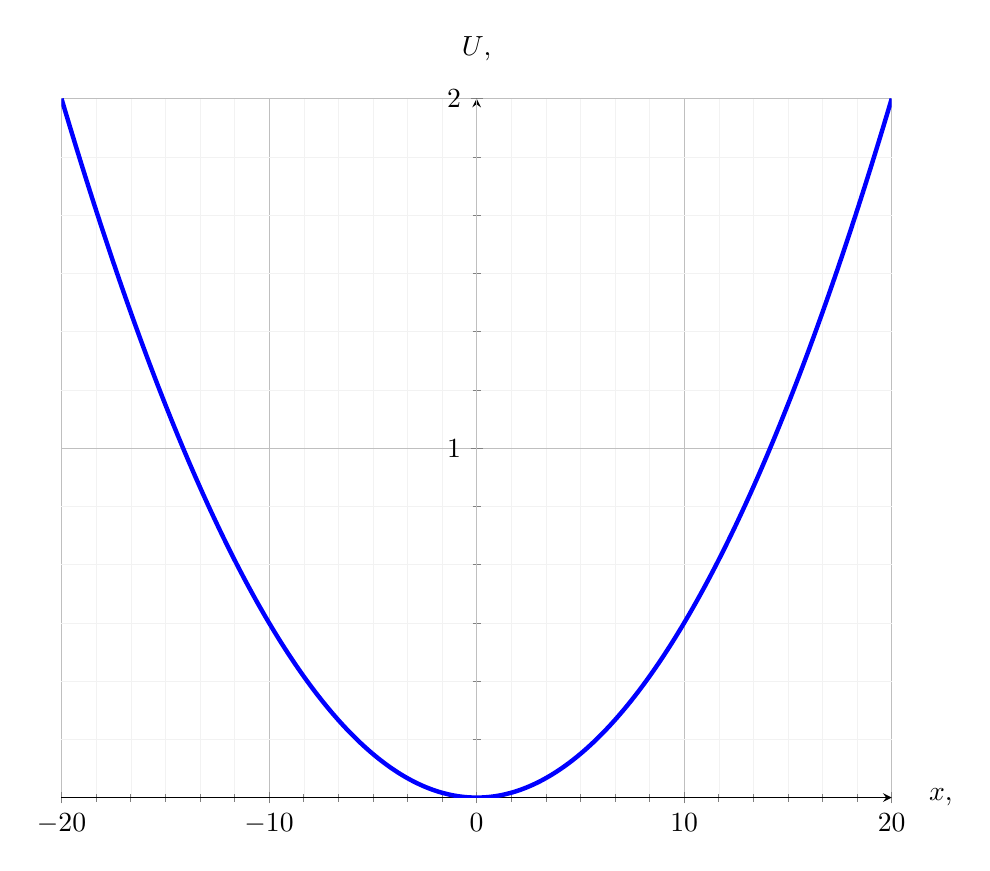
\begin{tikzpicture}
				\begin{axis}[%
					% === Налаштування сітки ===
					grid = both,
					grid style={line width=.1pt, draw=gray!10},
					major grid style={line width=.2pt,draw=gray!50},
					minor tick num = 5,
					minor grid style = {line width=.1pt,draw=gray!10},
					% === Налаштування положення координатних осей ===
					axis lines = middle,
					axis line style={-stealth},
					% === Вибір підписів шкали для відображення ===
					xtick = {-20,-10,...,20},
					extra x ticks=0,
					ytick = {0,1,2},
					% === Підпис координатних осей ===
					xlabel={$x$, \si{\centi\meter}},
					ylabel={$U$, \si{\joule}},
					% === Положення підпису координатних осей ===
					xlabel style={right = 10pt},
					ylabel style={above = 10pt},
					% === Налаштування мінімальних та максимальних значень координат ===
					xmin = -20,
					xmax =  20,
					ymin = 0,
					ymax =  2,
					% === Налаштування розміру графіка ===
					width=\linewidth,
					]
				\addplot+[blue, no marks, domain={-20:20}, samples=500, ultra thick] {0.005*x^2};
			\end{axis}
		\end{tikzpicture}
		\caption{Problem~\ref{prb:osc_U(x)}}
		\label{osc_U(x)}
	\end{minipage}
	%---------------------------------------------------------
	\begin{minipage}[t]{0.45\linewidth}\centering
		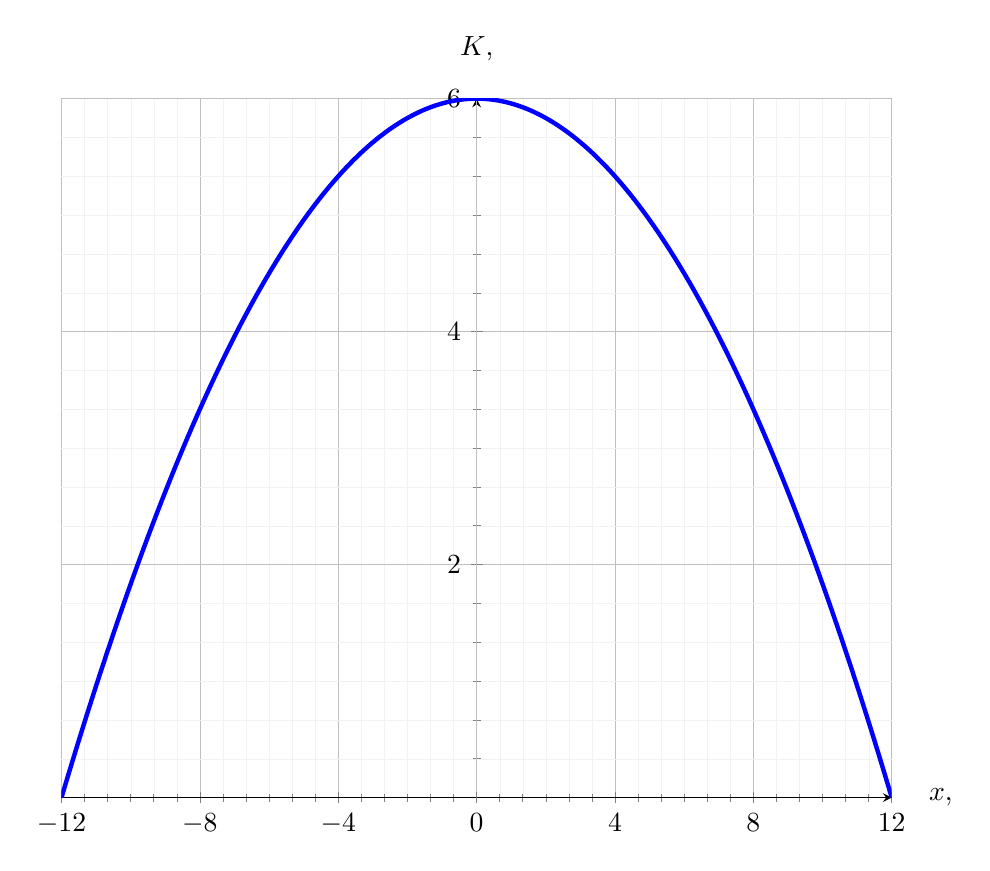
\begin{tikzpicture}
			\begin{axis}[%
				% === Налаштування сітки ===
				grid = both,
				grid style={line width=.1pt, draw=gray!10},
				major grid style={line width=.2pt,draw=gray!50},
				minor tick num = 5,
				minor grid style = {line width=.1pt,draw=gray!10},
				% === Налаштування положення координатних осей ===
				axis lines = middle,
				axis line style={-stealth},
				% === Вибір підписів шкали для відображення ===
				xtick = {-12,-8,...,12},
				extra x ticks=0,
				ytick = {0,2,4,6},
				% === Підпис координатних осей ===
				xlabel={$x$, \si{\centi\meter}},
				ylabel={$K$, \si{\joule}},
				% === Положення підпису координатних осей ===
				xlabel style={right = 10pt},
				ylabel style={above = 10pt},
				% === Налаштування мінімальних та максимальних значень координат ===
				xmin = -12,
				xmax =  12,
				ymin = 0,
				ymax =  6,
				% === Налаштування розміру графіка ===
				width=\linewidth,
				]
				\addplot+[blue, no marks, domain={-12:12}, samples=500, ultra thick] {6-(6/12^2)*x^2};
		\end{axis}
		\end{tikzpicture}
		\caption{Problem~\ref{prb:osc_K(x)}}
		\label{osc_K(x)}
	\end{minipage}
	%---------------------------------------------------------
\end{figure}
%=========================================================


%=========================================================
\begin{problem}\label{prb:osc_F(x)}
	A simple harmonic oscillator consists of a $0.50$~kg block attached to a spring. The block slides back and forth along a straight line on a frictionless surface with equilibrium point $x = 0$. At $t = 0$ the block is at $x = 0$ and moving in the positive $x$ direction. A graph of the magnitude of the net force $F$ on the block as a function of its position is shown in Fig.~\ref{osc_F(x)}. What are 
	\begin{enumerate*}[label=(\alph*)]
		\item the amplitude and
		\item the period of the motion,
		\item the magnitude of the maximum acceleration, and
		\item the maximum kinetic energy?
	\end{enumerate*}
	\begin{solution}
		\begin{enumerate*}[label=(\alph*)]
			\item $0.30$~m; 
			\item $0.28$~s; 
			\item $1.5 \cdot 10^2$~\si{\meter\per\square\second}; 
			\item $11$~J.
		\end{enumerate*}
	\end{solution}
\end{problem}


%=========================================================
\begin{problem}\label{prb:ocs_x(t)_en}
	Figure~\ref{ocs_x(t)_en} gives the position of a $20$~g block oscillating on the end of a spring.  What are 
	\begin{enumerate*}[label=(\alph*)]
		\item the maximum kinetic energy of the block and
		\item the number of times per second that maximum is reached?		
	\end{enumerate*}
(Hint: Measuring a slope will probably not be very accurate. Find another approach.)
	\begin{solution}
		\begin{enumerate*}[label=(\alph*)]
			\item $1.2$~J;
			\item $50$.
		\end{enumerate*}
	\end{solution}
\end{problem}

%=========================================================
\begin{figure}[h!]\centering
	%---------------------------------------------------------
	\begin{minipage}[t]{0.45\linewidth}\centering
		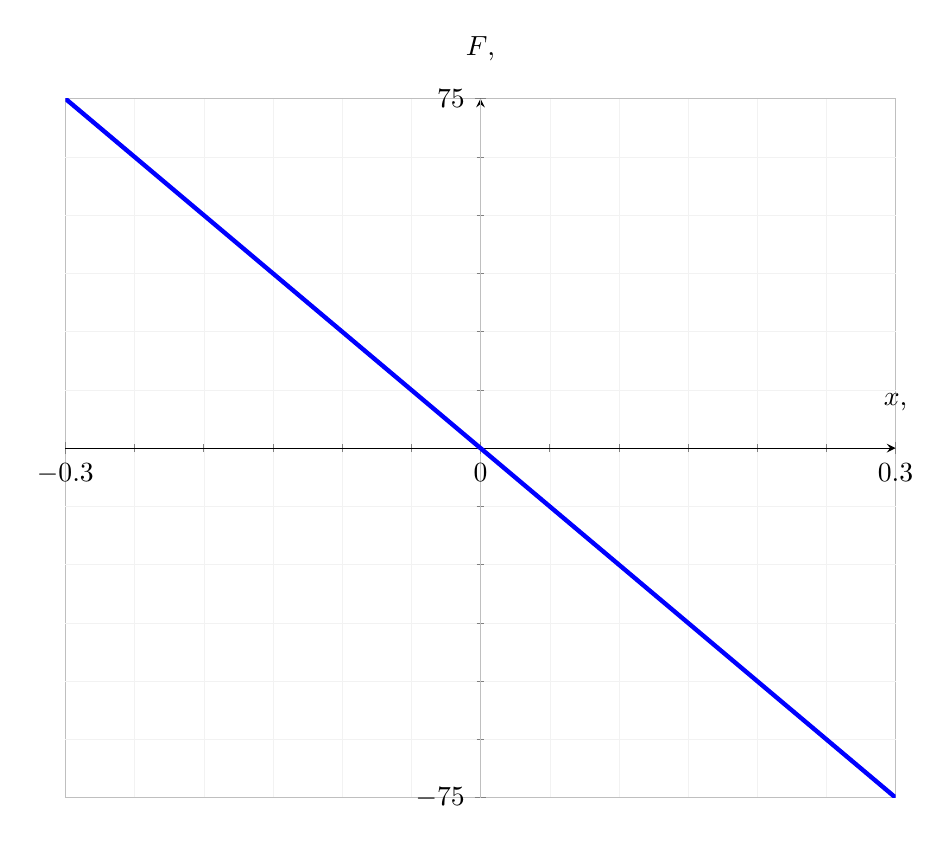
\begin{tikzpicture}
			\begin{axis}[%
			% === Налаштування сітки ===
			grid = both,
			grid style={line width=.1pt, draw=gray!10},
			major grid style={line width=.2pt,draw=gray!50},
			minor tick num = 5,
			minor grid style = {line width=.1pt,draw=gray!10},
			% === Налаштування положення координатних осей ===
			axis lines = middle,
			axis line style={-stealth},
			% === Вибір підписів шкали для відображення ===
			ytick = {-75,0,75},
			extra x ticks=0,
			xtick = {-0.30,0,0.30},
			% === Підпис координатних осей ===
			xlabel={$x$, \si{\meter}},
			ylabel={$F$, \si{\newton}},
			% === Положення підпису координатних осей ===
			xlabel style={above = 10pt},
			ylabel style={above = 10pt},
			% === Налаштування мінімальних та максимальних значень координат ===
			xmin = -0.30,
			xmax =  0.30,
			ymin = -75,
			ymax =  75,
			% === Налаштування розміру графіка ===
			width=\linewidth,
			]
			\addplot+[blue, no marks, domain={-0.30:0.30}, samples=50, ultra thick] {-250*x};
			\end{axis}
		\end{tikzpicture}
		\caption{Problem~\ref{prb:osc_F(x)}}
		\label{osc_F(x)}
	\end{minipage}
	%---------------------------------------------------------
	\begin{minipage}[t]{0.45\linewidth}\centering
		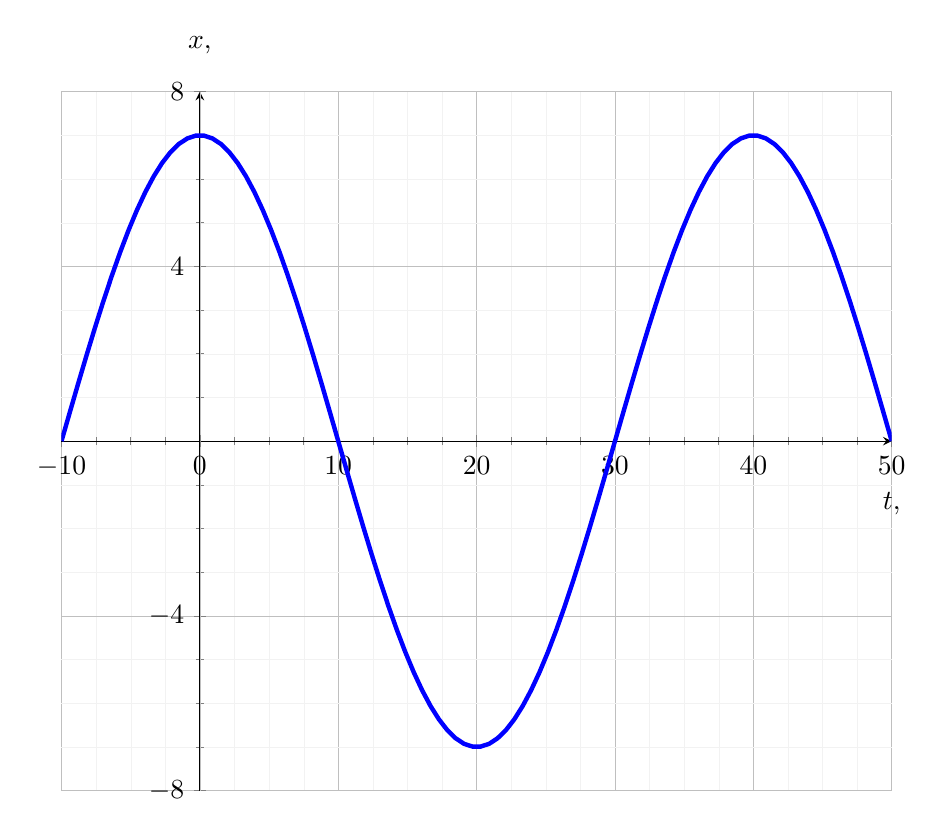
\begin{tikzpicture}
			\begin{axis}[%
			% === Налаштування сітки ===
			grid = both,
			grid style={line width=.1pt, draw=gray!10},
			major grid style={line width=.2pt,draw=gray!50},
			minor tick num = 3,
			minor grid style = {line width=.1pt,draw=gray!10},
			% === Налаштування положення координатних осей ===
			axis lines = middle,
			axis line style={-stealth},
			% === Вибір підписів шкали для відображення ===
			xtick = {-10,0,...,50},
			extra x ticks=0,
			ytick = {-8,-4,...,8},
			% === Підпис координатних осей ===
			xlabel={$t$, \si{\milli\second}},
			ylabel={$x$, \si{\centi\meter}},
			% === Положення підпису координатних осей ===
			xlabel style={below = 15pt},
			ylabel style={above = 10pt},
			% === Налаштування мінімальних та максимальних значень координат ===
			xmin = -10,
			xmax =  50,
			ymin = -8,
			ymax =  8,
			% === Налаштування розміру графіка ===
			width=\linewidth,
			]
			\addplot+[blue, no marks, domain={-10:50}, samples=100, ultra thick] {7*cos(deg(2*pi/40*x))};
			\end{axis}
			\end{tikzpicture}
			\caption{Problem~\ref{prb:ocs_x(t)_en}}
			\label{ocs_x(t)_en}
	\end{minipage}
	%---------------------------------------------------------
\end{figure}
%=========================================================


%=========================================================
\begin{problem}\label{prb:osc_bullet_hit_pendulum}
	A block of mass $M = 5.4$~kg, at rest on a horizontal frictionless table, is attached to a rigid support by a spring of constant $k = 6000$~N/m. A bullet of mass $m = 9.5$~g and velocity of magnitude $630$~m/s strikes and is embedded in the block (Fig.~\ref{osc_bullet_hit_pendulum}). Assuming the compression of the spring is negligible until the bullet is embedded, determine 
	\begin{enumerate*}[label=(\alph*)]
		\item the speed of the block immediately after the collision and
		\item the amplitude of the resulting simple harmonic motion.
	\end{enumerate*}
	\begin{solution}
		\begin{enumerate*}[label=(\alph*)]
			\item $1.1$~m/s; 
			\item $3.3$~cm.
		\end{enumerate*}
	\end{solution}
\end{problem}


%=========================================================
\begin{problem}\label{prb:osc_cylinder_on_spring}
	In Fig.~\ref{osc_cylinder_on_spring}, a solid cylinder attached to a horizontal spring ($k = 3.00$~N/m) rolls without slipping along a horizontal surface. If the system is released from rest when the spring is stretched by $0.250$~m, find 
	\begin{enumerate*}[label=(\alph*)]
		\item the translational kinetic energy and 
		\item the rotational kinetic energy of the cylinder as it passes through the equilibrium position.
		\item Show that under these conditions the cylinder's center of mass executes simple harmonic motion with period
	\end{enumerate*}
		\[
		T = 2\pi\sqrt{\frac{3M}{2k}},
		\]
	where $M$ --- is the cylinder mass. (Hint: Find the time derivative of the total mechanical energy.)
\end{problem}


%=========================================================
\begin{figure}[h!]\centering
	%---------------------------------------------------------
	\begin{minipage}[t]{0.45\linewidth}\centering
		\begin{tikzpicture}
		\node (ground) [ground,anchor=north,yshift=-0.2cm,minimum width=5cm,xshift=2.03cm] {};
		\draw (ground.north east) -- (ground.north west);
		
		\node (fill) [ground,xshift=-0.15cm,minimum height = 0.3cm, minimum width = 0.3cm] at (ground.west) {};
		
		\node (wall) [ground, rotate=-90, minimum width=1cm,anchor=south east] at (fill.north west) {};
		\draw (wall.north east) -- (wall.north west);
		
		\draw [fill=red!50] ([xshift=3cm]wall.north) coordinate  (mass) node[pt=black] {} circle (0.5) node[above=15pt] {$M$};
		
		\draw[-latex] (mass) +(-45:0.3) arc (-45:45:0.3);
		\draw [
		snake=coil,
		segment amplitude=5pt,
		segment length=5pt
		] (wall.north) -- node[above=5pt] {$k$} (mass);
		
		\end{tikzpicture}
		\caption{Problem~\ref{prb:osc_cylinder_on_spring}}
		\label{osc_cylinder_on_spring}
	\end{minipage}
	%---------------------------------------------------------
	\begin{minipage}[t]{0.45\linewidth}\centering
	\begin{tikzpicture}
		\node (ground) [ground,anchor=north,yshift=-0.2cm,minimum width=5cm,xshift=2.03cm] {};
		\draw (ground.north east) -- (ground.north west);
		
		\node (fill) [ground,xshift=-0.15cm,minimum height = 0.3cm, minimum width = 0.3cm] at (ground.west) {};
		
		\node (wall) [ground, rotate=-90, minimum width=1cm,anchor=south east] at (fill.north west) {};
		\draw (wall.north east) -- (wall.north west);
		
		\node [draw,minimum width=1cm,minimum height=1cm, fill=red!50] (mass) at ([xshift=3cm]wall.north) {$M$};
		
		\draw [
		snake=coil,
		segment amplitude=5pt,
		segment length=5pt
		] (wall.north) -- node[above=5pt] {$k$} (mass);
		
		\draw[-latex] ([xshift=5cm]wall.north) coordinate (B) -- +(-1,0) node[above] {$\vec v$};
		\fill[ball color = red] (B) circle (0.05); 
		\end{tikzpicture}
		\caption{Problem~\ref{prb:osc_bullet_hit_pendulum}}
		\label{osc_bullet_hit_pendulum}
	\end{minipage}
	%---------------------------------------------------------
\end{figure}
%=========================================================


\section{Period of Small Oscillations of Physicsl Pendulum}


%=========================================================
\begin{problem}\label{prb:osc_phys_pend_disk}
	In Fig.~\ref{osc_phys_pend_disk}, a physical pendulum consists of a uniform solid disk (of radius $R = 2.35$~cm) supported in a vertical plane by a pivot located a distance $d = 1.75$~cm from the center of the disk.The disk is displaced by a small angle and released. What is the period of the resulting simple harmonic motion?
	\begin{solution}
		$0.366$~\si{\second}.
	\end{solution}
\end{problem}


%=========================================================
\begin{problem}\label{prb:osc_phys_pend_rod}
	In Fig.~\ref{osc_phys_pend_rod}, a stick oflength $L = 1.85$~m oscillates as a physical pendulum. 
	\begin{enumerate*}[label=(\alph*)]
		\item What value of distance $x$ between the stick’s center of mass and its pivot point $O$ gives the least period?
		\item What is that least period?
	\end{enumerate*}
	\begin{solution}
		\begin{enumerate*}[label=(\alph*)]
			\item $0.53$~m; 
			\item $2.1$~s.
		\end{enumerate*}
	\end{solution}
\end{problem}


%=========================================================
\begin{figure}[h!]\centering
	%---------------------------------------------------------
	\begin{minipage}[t]{0.45\linewidth}\centering
		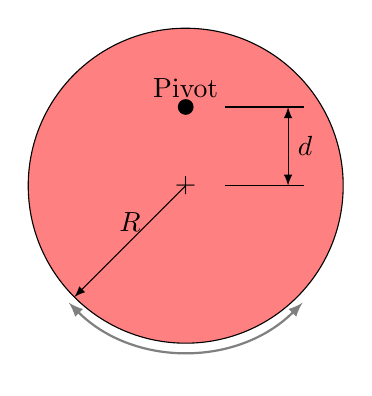
\begin{tikzpicture}
			\pgfmathsetmacro{\R}{2}
			\draw[fill=red!50] (0,0) circle (\R);
			\node at (0,0) {$+$};
			\draw[-latex] (0,0) -- node[above] {$R$} +(225:\R);
			\fill (0,\R/2) node[above] {Pivot} circle (0.1);
			\draw (0.5,\R/2)  -- +(1,0) coordinate[pos=0.8] (D1);
			\draw (0.5,0)  -- +(1,0) coordinate[pos=0.8] (D2);
			\draw[latex-latex] (D1) -- node[right] {$d$} (D2);
			\draw[latex-latex, thick, gray] (0,0) +(225:{\R+0.1}) arc (225:315:{\R+0.1});
		\end{tikzpicture}
		\caption{Problem~\ref{prb:osc_phys_pend_disk}}
		\label{osc_phys_pend_disk}
	\end{minipage}
	%---------------------------------------------------------
	\begin{minipage}[t]{0.45\linewidth}\centering
		\begin{tikzpicture}
			\node (ground) [ground,anchor=south, minimum width=4cm] {};
			\draw (ground.south east) -- (ground.south west);
			\begin{scope}[rotate=20]
				\draw[fill = red!50] (-0.1,1) rectangle +(0.2,-5) [add reference=P1];
				\node[pt = black] at (0,-2) {}; \node[below left] at (0,-2) {$C$};
			\end{scope}
			\node[pt = black] at (0,0) {}; \node[below left] at (0,0) {$O$};
			\draw[thick, dashed] (0,0) -- +(0,-4);
			\draw[latex-latex, thick, gray] (0,0) +({270-10}:3) arc({270-10}:{270+10}:3);
		\end{tikzpicture}
		\caption{Problem~\ref{prb:osc_phys_pend_rod}}
		\label{osc_phys_pend_rod}
	\end{minipage}
	%---------------------------------------------------------
\end{figure}
%=========================================================

%=========================================================
\begin{problem}
	A uniform circular disk whose radius $R = 12.6$~cm is suspended as a physical pendulum from a point on its rim.
	\begin{enumerate*}[label=(\alph*)]
		\item What is its period?
		\item At what radial distance $r < R$ is there a pivot point that gives the same period?
	\end{enumerate*}
\end{problem}

%=========================================================
\begin{problem}\label{prb:osc_cube_pend}
	The $3.00$~kg cube in Fig.~\ref{osc_cube_pend} has edgelengths $d = 6.00$~cm and is mounted on an axle through its center. A spring ($k  1200$~\si{\newton\per\meter}) connects the cube’s upper corner to a rigid wall. Initially the spring is at its rest length. If the cube is rotated 3 and released, what is the period of the resulting system?
\end{problem}


%=========================================================
\begin{problem}\label{prb:osc_pend_rod}
	In the overhead view of Fig.~\ref{osc_pend_rod}, a long uniform rod of mass $0.600$~kg is free to rotate in a horizontal plane about a vertical axis through its center. A spring with force constant $k = 1850$~\si{\newton\per\meter} is connected horizontally between one end of the rod and a fixed wall. When the rod is in equilibrium, it is parallel to the wall. What is the period of the small oscillations that result when the rod is rotated slightly and released?
	\begin{solution}
		$0.0653$~\si{\second}.
	\end{solution}
\end{problem}

%=========================================================
\begin{figure}[h!]\centering
	%---------------------------------------------------------
	\begin{minipage}[t]{0.45\linewidth}\centering
		\begin{tikzpicture}
			\node (wall) [ground, rotate=-90, minimum width=4cm,anchor=south east] at (fill.north west) {};
			\draw (wall.north east) -- (wall.north west);
			
			\coordinate (S) at ([yshift=1cm]wall.north); 
			
			\draw[fill = red!50, rotate around={45:(3,0)}] (3,0) rectangle +(2,2) [add reference = B];
			
			\fill (3,{2*cos(45)}) circle (0.1);
			\draw [
			snake=coil,
			segment amplitude=5pt,
			segment length=5pt
			] (S) node[pt=red] {}-- node[above=5pt] {$k$} (B north east) node[pt=red] {};
			
		\end{tikzpicture}
		\caption{Problem~\ref{prb:osc_cube_pend}}
		\label{osc_cube_pend}
	\end{minipage}
	%---------------------------------------------------------
	\begin{minipage}[t]{0.45\linewidth}\centering
		\begin{tikzpicture}
			\node (ground) [ground,anchor=south, minimum width=8cm] {};
			\draw (ground.south east) -- (ground.south west);
			\coordinate (S) at ([xshift=1cm]ground.south west); 
			\node[pt=red] at (S) {};
			\draw[fill=red!50, rotate around = {10:(0,-2)}] (-3,{-2-0.1}) rectangle +(6,0.2) [add reference = B];
			\node[pt=black, pin={[pin edge={black, -}]-60:Rotation axis}] at (0,-2) {};
			\draw [
			snake=coil,
			segment amplitude=5pt,
			segment length=5pt
			] (S) -- node[left=5pt] {$k$} (B west) node[pt=red] {};
		\end{tikzpicture}
		\caption{Problem~\ref{prb:osc_pend_rod}}
		\label{osc_pend_rod}
	\end{minipage}
	%---------------------------------------------------------
\end{figure}
%=========================================================

\section{Damped Oscillations}


%=========================================================
\begin{problem}
	The amplitude of a lightly damped oscillator decreases by 3.0\% during each cycle. What percentage of the mechanical energy of the oscillator is lost in each cycle?
	\begin{solution}
		$7\%$.
	\end{solution}
\end{problem}


%=========================================================
\begin{problem}
	A point performs damped oscillations with frequency co and damping coefficient $\beta$. Find the velocity amplitude of the point as a function of time $t$ if at the moment $t = 0$
	\begin{enumerate*}[label=(\alph*)]
		\item its displacement amplitude is equal to $a_0$;
		\item the displacement of the point a $0$ and its velocity projection $v_0$.
	\end{enumerate*}
	\begin{solution}
		\begin{enumerate*}[label=(\alph*)]
			\item $v = a_0\sqrt{\omega^2 + \beta^2}e^{-\beta t}$;
			\item $v = |v_0|  \sqrt{1 +  \left( \frac{\beta}{\omega}\right)^2}e^{-\beta t}$.
		\end{enumerate*}	
	\end{solution}
\end{problem}


%=========================================================
\begin{problem}
	For the damped oscillator system, the block has a mass of $1.50$~kg and the spring constant is $8.00$~N/m. The damping force is given by $-b(dx/dt)$, where $b = 230$~g/s. The block is pulled down $12.0$~cm and released. 
	\begin{enumerate*}[label=(\alph*)]
		\item Calculate the time required for the amplitude of the resulting oscillations to fall to one-third of its initial value. 
		\item How many oscillations are made by the block in this time?
	\end{enumerate*} 
	\begin{solution}
		\begin{enumerate*}[label=(\alph*)]
			\item $14.3$~s; 
			\item $5.27$.
		\end{enumerate*}
	\end{solution}
\end{problem}


\section{Forced Oscillations and Resonance}


%=========================================================
\begin{problem}
	A $2.00$~kg object attached to a spring moves without friction and is driven by an external force given by the expression $F = 3.00\sin(2\pi t)$, where $F$ is in newtons and $t$ is in seconds. The force constant of the spring is $20.0$~N/m. Find 
	\begin{enumerate*}[label=(\alph*)]
		\item the resonance angular frequency of the system,
		\item the angular frequency of the driven system,
		and
		\item the amplitude of the motion.
	\end{enumerate*}
	\begin{solution}
		\begin{enumerate*}[label=(\alph*)]
			\item $3.16$~\si{\per\second}; 
			\item $6.28$~\si{\per\second};
			\item $5.09$~cm.
		\end{enumerate*}
	\end{solution}
\end{problem}


%=========================================================
\begin{problem}
	A block weighing $40.0$~N is suspended from a spring that has a force constant of $200$~N/m. The system is undamped and is subjected to a harmonic driving force of frequency $10.0$~Hz, resulting in a forced-motion amplitude of $2.00$~cm. Determine the maximum value of the driving force.
\end{problem}


%=========================================================
\begin{problem}
	Damping is negligible for a $0.150$~g object hanging from a light, $6.30$~N/m spring. A sinusoidal force with an amplitude of $1.70$~N drives the system. At what frequency will the force make the object vibrate with an amplitude of $0.440$~m?
	\begin{solution}
		$0.641$~Hz or $1.31$~Hz.
	\end{solution}
\end{problem}

\section{Superposition of Harmonic Oscillations}

\subsection{Superposition of Harmonic Oscillations of the same direction}

%=========================================================
\begin{problem}
	Two simple harmonic oscillations are represented by 
	\begin{align*}
		x_1 &= 3\sin(20\pi t + \nfrac{\pi}{6}) \\
		x_2 &= 4\sin(20\pi t + \nfrac{\pi}{3})
	\end{align*}
	Find the 
	\begin{enumerate*}[label=(\alph*)]
		\item amplitude,
		\item phase constant and
		\item the period of resultant vibration.
	\end{enumerate*} 
\end{problem}


%=========================================================
\begin{problem}
	The superposition of two harmonic oscillations of the same 
	direction results in the oscillation of a point according to the law 
	$x  = a\cos(2.1 t) \cos 50.0 t$, where $t$ is expressed in seconds. Find the
	\begin{enumerate*}[label=(\alph*)]
		\item angular frequencies of the constituent oscillations and
		\item the period with which they beat. 
	\end{enumerate*} 
	\begin{solution}
		\begin{enumerate*}[label=(\alph*)]
			\item $47.9$~\si{\per\second} and $52.1$~~\si{\per\second};
			\item $1.5$~\si{\second}.
		\end{enumerate*}
	\end{solution}
\end{problem}

\subsection{Superposition of of Harmonic Oscillations of the mutually perpendicular directions}


%=========================================================
\begin{problem}
	Find the trajectory equation $y(x)$ of a point if it moves  
		according to the following laws: 
		\begin{align*}
			x &= a\sin(\omega t) \\
			y &= a\sin(2\omega t)
		\end{align*}
	Plot these trajectories. 
	\begin{solution}
		$y^2 = 4x^2 (1 - \frac{x^2}{a^2})$.
		
		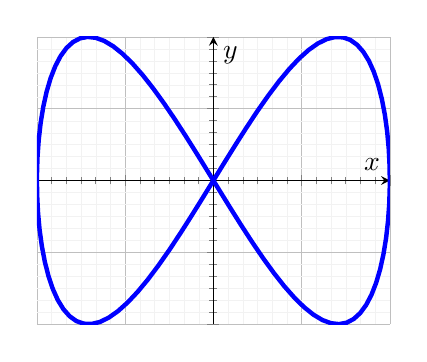
\begin{tikzpicture}
		\begin{axis}[%
		% === Налаштування сітки ===
		grid = both,
		grid style={line width=.1pt, draw=gray!10},
		major grid style={line width=.2pt,draw=gray!50},
		minor tick num = 5,
		minor grid style = {line width=.1pt,draw=gray!10},
		% === Налаштування положення координатних осей ===
		axis lines = middle,
		axis line style={-stealth},
		xticklabels = \empty,
		yticklabels = \empty,
		xlabel={$x$},
		ylabel={$y$},
		width=0.5\linewidth,
		trig format plots=rad,
		]
		\addplot [domain=0:2*pi, samples=100, blue, ultra thick] ({1*sin(x)}, {1*sin(2*x)});
		\end{axis}
		\end{tikzpicture}
	\end{solution}
\end{problem}

%=========================================================
\begin{problem}
	Find the trajectory equation $y(x)$ of a point if it moves  
	according to the following laws: 
	\begin{align*}
	x &= a\sin(\omega t) \\
	y &= a\cos(2\omega t)
	\end{align*}
	Plot these trajectories. 
	\begin{solution}
		$y^2 = a (1 - \frac{2x^2}{a^2})$.
		
		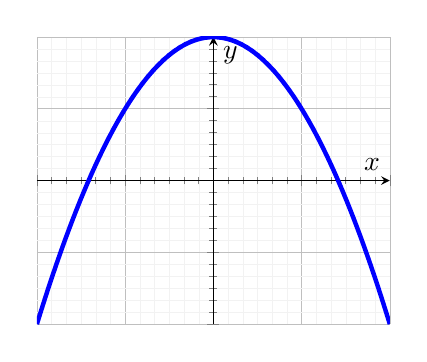
\begin{tikzpicture}
		\begin{axis}[%
		% === Налаштування сітки ===
		grid = both,
		grid style={line width=.1pt, draw=gray!10},
		major grid style={line width=.2pt,draw=gray!50},
		minor tick num = 5,
		minor grid style = {line width=.1pt,draw=gray!10},
		% === Налаштування положення координатних осей ===
		axis lines = middle,
		axis line style={-stealth},
		xticklabels = \empty,
		yticklabels = \empty,
		xlabel={$x$},
		ylabel={$y$},
		width=0.5\linewidth,
		trig format plots=rad,
		]
		\addplot [domain=0:2*pi, samples=100, blue, ultra thick] ({1*sin(x)}, {1*cos(2*x)});
		\end{axis}
		\end{tikzpicture}
	\end{solution}
\end{problem}

\Closesolutionfile{answer}

